\documentclass[preprint]{elsarticle}
\biboptions{round, numbers}
\usepackage[latin1]{inputenc}
%\usepackage[T1]{fontenc}
%\usepackage{textcomp}
\usepackage{graphicx}
\usepackage{color}
%\usepackage{setspace}
\usepackage{url}
\usepackage[english]{babel}

\begin{document}

\begin{frontmatter}

%%%%%%%%%%%%%%%%%%%%%%%%%%%%%%%   TITLE   %%%%%%%%%%%%%%%%%%%%%%%%%%%%%%%

\title{Corporate Security Solutions for BYOD:\\ A Novel User-Centric and Self-Adaptive System}

%%%%%%%%%%%%%%%%%%%%%%%%%%%%%%%   AUTHORS   %%%%%%%%%%%%%%%%%%%%%%%%%%%%%%%

\author{P. de las Cuevas, A.M. Mora, J.J. Merelo,\\ P. Garc�a-S�nchez, A. Fern�ndez-Ares}
\ead{\{paloma, amorag, jmerelo, pgarcia, antares\}@geneura.ugr.es}
\address{Departamento de Arquitectura y Tecnolog�a de Computadores.\\ ETSIIT - CITIC. University of Granada, Spain}
%\author{A. M. Mora}
%\ead{amorag@geneura.ugr.es}
%\address{Departamento de Arquitectura y Tecnolog�a de Computadores. Escuela T�cnica Superior de Ingenier�as Inform�tica y de Telecomunicaci�n. CITIC. University of Granada, Spain}

%\maketitle

%
%%%%%%%%%%%%%%%%%%%%%%%%%%%%%%%%%   ABSTRACT   %%%%%%%%%%%%%%%%%%%%%%%%%%%%%%%%%
%
\begin{abstract} 
Enterprises, and particularly their Chief Security Officers (CSOs),
want to ensure that their Security Policies are complied, but this
goal turned hard to achieve since employees are able to use, or bring,
their personal devices at work. This has been named as ``Bring Your Own Device'' (BYOD). % <- Problem
As this BYOD philosophy is being adopted by many companies everyday, a number of solutions have appeared in the market, 
in order to adapt to it in a secure way. In this paper, a novel and open source system named
MUSES (Multiplatform Usable Endpoint Security), able 
to securely manage BYOD environments, is described. % <- Solution
MUSES has been developed to cope with security issues with regard to enterprise security policies, but as a user-centric tool. It considers users' behaviour in order to adapt, improve, or even increase the defined set of security rules. To do this, the system applies Machine Learning and Computational Intelligence techniques, being also able to predict future security incidences produced by these users. % <- Solution, details.
MUSES, which has released its first prototype this year, is compared with the most relevant
solutions offered by other companies to deal with the same issues as, remarking the advantages that our system offers with
respect to them. % <- we will explain why is better in the work

% What do we do in this paper? Present the
                 % architecture? The prototypes? - JJ
\end{abstract}

%FERGU: seguro que ya lo hab�is discutido, pero presentar MUSES como algo a hacer en el futuro es un poco... yasabesh xD

%
%%%%%%%%%%%%%%%%%%%%%%%%%%%%%%%%%   KEYWORDS   %%%%%%%%%%%%%%%%%%%%%%%%%%%%%%%%%
%
\begin{keyword}
Corporate mobile security \sep End-to-end security solutions \sep User-centric systems \sep Self-adaptation \sep Multiplatform \sep Security Policies \sep Data security and data privacy \sep BYOD
\end{keyword}

\end{frontmatter}


%-------------------------------------------------------------------------------
%%%%%%%%%%%%%%%%%%%%%%%%%%%%%%%   INTRODUCTION   %%%%%%%%%%%%%%%%%%%%%%%%%%%%%%%
%-------------------------------------------------------------------------------

\section{Introduction}
\label{sec:intro}

The way how users have used their devices has changed in the past few years, even the number of different devices per user is increasing because of the so-called Internet of Things \cite{weber2010internet}. Thanks to it, users have more flexibility, and also at their works, because now they can use their devices to access company assets and continue working outside of the workplace. To allow this way of working, companies started to adopt what has been called the Bring Your Own Device (BYOD) philosophy.

Data security and privacy are key factors for a company, and thus, in
order to protect them, it is usual that the Chief Security Officer (CSO) of a company defines a set of Organisational Security
Policies \cite{Opp_Security11}. However, allowing a BYOD environment means to take care of the risks that the use of personal smartphones can bring to the company \cite{gangula2013survey}. For instance, the mixture between personal and professional information in these devices would allow the user to navigate inside social networks, where important data could be leaked in the event of a security incident. 

In this scenario several solutions have appeared in order to manage corporate security. Most of the solutions are focused for both smartphones and desktop PCs, although some are implemented for a certain platform. However, almost all of them try to be non-intrusive -with regard to users' personal data-, friendly, and easy to use. 

Moreover, it has been demonstrated that employees who ignore company security policies are the main hazard for company security \cite{Adams_Users05}. In this situation, the tools that are appearing in the market aim to cope with the concept of seamless working experience on different devices. This concept is a methodology of work which allows users to start, or continue a working session, over multiple devices and locations, without any significant loss of data. This new situation has a big impact from the point of view of the security \cite{Schu_SecPatterns05}, since company data borders have changed in the last years. Therefore, now the users can access important data from outside the enterprise, and possibly through a non completely secure channel. %Antares - Yo quitaba lo de significant loss of data, ya que significant se repite despu�s.
%Cambiado

This work introduces a recently released system named
MUSES, from Multiplatform Usable Endpoint Security, which is a
dev\-ice\--in\-de\-pen\-dent end-to end user-centric tool, based on a
set of security rules defined as specifications of the Corporate
Security Policies. In addition, it has the ability of `learning' from the user's past behaviour and adapt the set of existing rules, or even inferring new ones,
in order to deal with potential security incidents that they might cause in the future. 
Then the system reacts, in a non-intrusive way, to the potentially
dangerous sequence of actions \footnote{Which are treated as `events' inside the system.} that the employees are conducting at
any time. The MUSES system has been also tested in an actual company, with satisfactory results. The analysis of all data from these tests, and conclusions, are part of the future work.


To this end, MUSES analyses the users' behaviour by means of Data
Mining (DM) techniques \cite{DataMining_Lee01} and Machine Learning
(ML) methods \cite{MachineLearning_Bishop06}, extracting a set of
patterns which is later processed by means of Computational
Intelligence (CI) algorithms, namely Evolutionary Computation methods
\cite{EAs_Back96,GP_Koza92}. The general ideas behind MUSES were
already presented in
\cite{DBLP:conf/sac/MoraCGZJEBAH14,DBLP:conf/gecco/MoraCGZE14}. However,
the implementation was in its early stages when those papers were
submitted. Also, an additional work on the data mining techniques was conducted in \cite{mora14:urls}, over a set of data previous to the release and test of the first MUSES prototype. As there was no available test data, a set of URL connection logs were provided by a Spanish company, as well as both black and white lists. These lists contained the URLs that were forbidden, or allowed, to be accessed by the employees. By taking the lists as `rules', and the HTTP connections as `events', a previous simulation of the rule generation through classification, and its results, could be presented at \cite{mora14:urls}. Now, after the release of the first prototype, along with the first conducted tests, we have a clearer idea of MUSES capabilities and, as such, they will be presented in this paper. 


MUSES includes some important modules in its core, %FERGU: no hab�is hablado de ese loop, decid mejor "core" (no lo cambio yo por si no tiene sentido)
%cambiado
 such as an Event Processor, which performs an event correlation task \cite{SurveyEventCorrelation_Tiffany02}, matching occurred events with rules to deal with them, and extracting threats that a Real-Time Risk and Trust Analysis Engine (RT2AE) \cite{RT2AE_SOTICS13} will process (along with other trust data and profiles), to select the best subset of policies.

But first, this work presents a brief overview of the main existing solutions in this environment. Then, a comparison between these tools and MUSES is also conducted, focusing on the advances beyond the state of the art that this novel system (being developed inside an European Project\footnote{\url{http://musesproject.eu/}} of the same name) includes . 


The rest of the paper is organized as follows. First, some background situation about enterprise security is presented in Section \ref{sec:preliminaryconcepts}, explaining how BYOD philosophy affects it. Then, the main tools/solutions are detailed in Section \ref{sec:toolsreview}, even if they are still in development.  
Then, in Section \ref{sec:muses}, the Multiplatform Usable Endpoint Security System is presented (architecture + soft computing techniques). Its advantages and benefits in comparison with the other solutions are commented in Section \ref{sec:comparison}.
Finally, the reached conclusions are discussed in Section \ref{sec:conclusions}.


%----------------------------------------------------------------------------
%%%%%%%%%%%%%%%%%%%%%%%%%%%%%%%   BACKGROUND  %%%%%%%%%%%%%%%%%%%%%%%%%%%%%%%
%----------------------------------------------------------------------------


\section{Preliminary concepts and background about enterprise security}
\label{sec:preliminaryconcepts}

One of the tasks of a Chief Security Officer (CSO) is to elaborate an efficient set of Information Security Policies (ISPs), for controlling a certain, and already known, structure \cite{Opp_Security11}. This means that, until the appearance of BYOD, enterprises used to follow static security policies devoted to control an environment where the company assets and the devices were purchased and maintained by the company. Now that corporate networks are becoming dynamic for being adapted to this BYOD philosophy, there is an additional risk because the devices that the employees use are not always company-owned. This means that the CSOs have to find the balance between having a fast response to any user action that might cause harm (in terms of money loss because of a security incident), and trying to avoid monitoring the users in a way that is against privacy. A needed security policy, or in this case, an ISP should deal with the way of protecting a certain organization's information against a security breach. Though there are standards, such as the ISO27002 or the Security Forum's Standard of Good Practice\footnote{\url{https://www.securityforum.org}}, and many guidelines \cite{SecPol09}, an ISP should be adapted depending on the characteristics of the community/organisation that they are built for. In this sense, MUSES stands up for a self-adaptation of the security policies of a company.

On the other hand, employee-owned devices like smartphones, can be both used for personal matters at work, and for continuing working outside of the workplace. As the name says, smartphones are more than simple mobile phones, and people who use them in their works have the possibility of maintaining a good balance between work and private life. For this reason, the risk of uncontrolled devices accessing to corporate assets in unsafe conditions, due to the number of new risks which are linked to smartphones \cite{gangula2013survey}, is bigger.

Normally, the enterprise network architecture was being adapted to cope with external attackers \cite{MIT05}. With the incorporation of BYOD, the threat is about corporate assets being compromised due to employees' devices with vulnerabilities \cite{android11}, or leaked because they are being accessed from a device connected through an insecure (public) network.

Thus now, more risky situations should be considered when designing a company's network architecture. In Figure \ref{fig:proposed_diagram} there is a proposal which can be used for the beginning of the study of solutions that may secure such a dynamic environment. It includes the possibility of having employee-owned mobile (smartphones and tablets) and portable (laptops) devices, and also the opportunity that the employees have of connecting these devices either from inside or outside the company premises. Moreover, company's information assets are constantly accessed under these conditions, considering that an information asset means every \textit{piece of information} that has a \textit{value} (cost depending on the risk of being lost or leaked) for the company. It can be referred to files with sensitive information, as well as confidential mails, or even to company applications.

\begin{figure}[ht]
	\begin{center}
		\includegraphics[scale=0.4]{img/proposed_diagram.eps}
		\caption{Architecture approach of an enterprise network, assuming that it has adopted the BYOD philosophy.}
	\label{fig:proposed_diagram}
	\end{center}
\end{figure}

The other issue to cope with is the elaboration of a good ISP, understandable for every user of the company, and more importantly, non-intrusive for him. A lot of researchers have studied the natural tendency of employees to comply with the ISP \cite{SecPolComp10,SecPolComp12,SecPolComp14}, reaching conclusions such as the employees compliance with the security policies increases educating/training them in information security awareness  \cite{SecPolComp09}, and decreases applying too much sanctions when a misuse or abuse occurs \cite{SecPolPenalty09}. Thus, in this paper, for each tool in Section \ref{sec:toolsreview} it is specified if the developers have taken into account the construction of ISPs, or even if they give some guidelines for building them.

This situation leads to a need of protecting the organisation's side, but also the users' side, making non-interfering easy-to-follow ISPs, and leaving them to use their devices for personal purposes while working, without putting organisation's information assets under risk. The compliance of these requirements would compose an End-to-End Security Solution (protecting both enterprise and employee), which is the motivation of the commented tools and, as presented in Section \ref{sec:muses}, is the aim of the MUSES project.


%------------------------------------------------------------------------------
%%%%%%%%%%%%%%%%%%%%%%%%%%%%%%%   TOOLS REVIEW  %%%%%%%%%%%%%%%%%%%%%%%%%%%%%%%
%------------------------------------------------------------------------------

\section{Tools for corporate mobile security}
\label{sec:toolsreview}

Many tools for companies, as well as for devices, which have adopted the BYOD have been released in the past four years. This way, and
more focused on the enterprise, there are some tools which offer the CSO ways to control the devices which enter into the system, for instance, and also to protect the employees' data by means of data encryption and data protection by requiring the use of strong and secure passwords. Other tools for managing a BYOD situation add to their features guidelines for the CSOs to develop good ISPs. On the other hand, many solutions have been presented which are more focused on the device side, although they implement also the server side. Some of those tools have influenced the development of the MUSES system  itself (Section \ref{sec:muses}), which can complement them, as adds other features that go beyond the state of the art. The present section introduces the most relevant features of these products, as they can be considered related to the MUSES objectives.

%----------------------------------------------------------------------------

\subsection{IBM Mobile Security}
\label{subsec:ibm}

One of the first companies who supported the BYOD model was IBM \cite{IBM_tool}, as they recognized the increase of employees who brought their personal smartphones or tablets into the workplace \cite{ibm11}. IBM has different solutions divided into ``technology solutions'', and ``services'', and almost all are are mainly focused on the management of the devices in the system. Then, it might seem clear that the first disadvantage is not including all features in one system, but to make the companies to choose between one or another, or invest even more resources instead.

Having a look into what IBM offers as ``services'', three services can be found:

\begin{itemize} 
	\item \textit{Mobile Enterprise Services}: Is offered as an integrated solution for smartphones, and tablets as well, but then it is divided in different subservices that the company has to acquire separately. Some of them are related to cloud computing, such as events and log management as a cloud security service, cloud backup, or the so-called `hosted vulnerability management'. The last one is specially interesting for the scope of this paper, given the fact that it seems to implement one of the most important advantages of the MUSES system, the self-adaptation. IBM, by performing deeper scans over the security incidents data, either if they were successful (computer forensics analysis) or not (the device was enough secure), they claim to be able to recognise new vulnerabilities - or threats - with enough accuracy. The main difference with MUSES in this case, is that MUSES includes this feature in the system, without the need of purchasing the service separately, and configuring the different parts. Also, the fact that IBM software is not open source as MUSES system is, to verify the success of this feature is highly difficult, as they do not present statistics in their website either.
	\item \textit{Hosted Mobile Device Security Management}: A particular service of the Mobile Enterprise Services. It includes itself a number of subservices, going from tools to make easy to develop secure mobile apps, to an interface for managing the devices in the system, checking their configuration security level. Again, what is offered by IBM as `services', are included as default features in the MUSES system.
	\item \textit{Enterprise Wireless Networks}: Devoted to provide secure channels for communications. This is related to ensuring employees that any connection they might perform to access company assets, is properly secured, at the time it delivers the expected performance. Thus, this service is, in some sense, adaptive to the situation, yet only in terms of a secure connection and not evolving the security policies, like MUSES. 
\end{itemize}

%----------------------------------------------------------------------------

\subsection{Sophos Mobile Control}
\label{subsec:sophos}

Contrarily to IBM's solution services, Sophos offers a whole product for securing BYOD environments, which is called Mobile Control \cite{Sophos_tool}. It is oriented to IT administration for mobile devices, and it can be deployed in two ways: on-premises, which means that all data and services remain in the servers of the company, and as Software as a Service (SaaS), so that the services are provided through Lightweight Directory Access Control (LDAP). LDAP is an application protocol for accessing and maintaining distributed directory information services over an Internet Protocol (IP) network.

The tool manages all employees' smartphones and tablets from a single-based console. This console monitors the devices since the initial set up and registration, until they log off. Other features are similar to IBM's product, adding some new such as the incorporation of a service called Malware and Web protection, so that there is no need for having a previously installed antivirus in the devices.

With regard to compliance enforcement, the main goal of this Mobile Control tool is to give more importance to company security, instead of giving more flexibility to the users. But it has been demonstrated by Herath and Rao in \cite{SecPolPenalty09} that this practise can result in bad (even not on purpose) users' behaviour. Thus, the company BYOD initiative should include an acceptable use policy to ensure that the users are aware of the measures that the company would take if a device breaches any ISPs. Sophos aims to reach this by doing three main tasks: First, by allowing setting up user and group-based security policies separately. Secondly, by a risk mitigation in which the actions to perform can be set according to the severity of the breach. For minor cases, the company may want to simply inform to the user, but if sensitive data is at risk, a remote wipe may be the chosen option. Finally, compliance check, by constantly performing scans to detect malware and putting the devices in quarantine when they are found infected.

Thus, given the fact that this tool is more focused on the company than in the user, it is worth to compare it to the MUSES system, as the latter tries to focus on the users, being user-centric. This means that is preferred to let the user know about a risky situation, rather than making them feel ``watched''.

%----------------------------------------------------------------------------

\subsection{Samsung KNOX and Blackberry Balance}
\label{subsec:samsungblackberry}

Even though these two tools are provided by two different manufacturers, Samsung and Blackberry, they both have in common their situation. They are not being successful in spite of their features. On the one hand, Blackberry sales have been decreasing since 2010 \cite{Blackberry_sales}. 
On the other hand, Samsung revealed at the Barcelona Mobile World Congress 2013 the KNOX application \cite{Samsung_mwc13}, which was expected to be available on its last Galaxy smartphone generation. Then, it was delayed and again presented in the same congress in 2014 \cite{Samsung_mwc14}, but still semained delayed until it was apparently found insecure \cite{Samsung_insecure}. Finally, Samsung decided to collaborate with Google in Android Work \cite{Samsung_android} (see Section \ref{subsec:androidwork}).

With regard to their features, Samsung KNOX, as well as Blackberry Balance, are more focused on the device side, while the solutions mentioned in previous subsections were more centered in being tools for CSOs. This also means that they are not device-independent, as KNOX is only for Samsung devices and Balance is integrated in BlackBerry 10 \cite{Blackberry_tool}.

The main feature of KNOX is the use of different containers, or environments, for business and personal sides. Each one even includes its own graphical configuration (wallpapers, colours, and so on), in order to be more easily recognised and distinguished by the user.
A password is required in order to enter into the business side and, once \textit{logged in} in this container, no more passwords are needed for the business applications. The applications approved by the company IT department must meet Samsung security standards and, though it has been said that KNOX is a device-focused solution, it offered an API. This API would allow the company to access to over almost 205 predefined IT policies. With regard to information protection methods, data files saved by applications of each environment are encrypted with AES 256-bit algorithm, in such manner that only the appropriate container can access these files. In the same way, the user is not allowed to share data between the two environments. 

Features in Blackberry Balance are similar. This security package was announced as a feature of BlackBerry 10. Nevertheless, it is available with BlackBerry Enterprise Service 10, which is a device management, security and app management for BlackBerry, iOS and Android devices. It is necessary to activate BlackBerry Balance for having available some security features, all related or similar to the aforementioned. For instance, a message is displayed when the user tries to copy work data and then paste it into personal apps. Also, a user attempting for actions that are not permitted in the company ISP, or may cause secure work information to be in contact with personal applications, these actions will not be permitted. 

On the other side, employees are able to access information and applications related to their personal lives, while staying connected to important work information when they need to perform. Finally, another known feature is also offered by Blackberry, so if the device gets lost or is stolen, or if the employee leaves the organization, there will be an option to wipe just work information which can be done remotely.

As a summary, Blackberry Balance has little opportunity if Blackberry sales continue to decrease, as well as Samsung KNOX, which is still out of the market. With this situation, MUSES could be a good choice, because is device-independent, and is available as an open source tool for both devices and servers.

%----------------------------------------------------------------------------

\subsection{Blackphone}
\label{subsec:blackphone}

On the device side, one of the most powerful solutions found in the BYOD state of the art seems to be to directly use a phone which has been developed with data security in mind such as the BlackPhone \cite{Blackphone}. It has its own Android-based operating system, called \textit{PrivatOS}, which includes a privacy-focused application store (called \textit{Silent Store}) that takes care of the problem of applications which ask for certain permissions that can lead, for instance, to personal data leakage \cite{gangula2013survey}. This BlackPhone also allows a remote wiping of the data if the device is lost or stolen. The main disadvantage of this solution is either the enterprise having to make
an investment and buy these smartphones to the employees (which, in fact, is against the BYOD philosophy), or to make employees buy them,
so they cannot use the device they already have. On the contrary, the MUSES system proposed in this work is designed as device-independent.

%----------------------------------------------------------------------------

\subsection{Android Work}
\label{subsec:androidwork}

This tool is the Google approach in the mobile enterprise security area, and  will run on Android 5.0 ``Lollipop''. It follows the idea of containers, previously presented in the Samsung KNOX description. Thus the container will be used to manage (encrypted) corporate data, and also to restrict what the users can do with them. This is called a ``dual-persona'' smartphone \cite{AndroidWork_review}.

This system will be strongly related to the Google Play market, as the applications will be `categorized'. Thus, Android Work will provide the CSOs with a tool to define which apps would be allowed for being installed by the users and considered as corporate-related applications. Several enterprise-security aimed applications will be offered in the market, so the IT would decide which ones will be installed (even as a bundle) in the employees' devices, and also, they can manage the updates of these apps, in order to ensure that all the employees are up to date. For instance, one app could manage the creation of personal/work profiles, so the user just could access corporate assets after login in into the app. Moreover, the enterprise IT department could define specific security policies on these apps, in addition to the inherent protection that the container provides. However, the specifications of this tool \cite{AndroidWork_tool} do not include the ``self-adaptation'' as a feature, as the MUSES system does. 

Even though it does not analyse the system information for security rules evolution purposes, it offers policy management. Thus, the system will provide a framework for IT staff to manage business devices, but also, and more importantly, personal devices being used in a BYOD context (The CSO would give the employee an activation code in order to `connect' the smartphone to the enterprise and use this Android Work).
Therefore, IT admins will be able to specify which Google Play apps will be available for users to install through this work profile, including being able to provision apps to specific individuals or groups (inside the company).

In addition to the work profiles, there will be considered other high-level ones with the ability to administrate the device from the corporate-security point of view, or as the owner, with all the privileges on the device.

Android work has only one advantage over MUSES, and roughly over all solutions, which is the ability to act over the Android kernel. All the other tools only have permission for monitoring the running processes in the devices, while Android work has, for instance, the ability to provide a `work' version of its native apps. MUSES, instead, depends on if the developers adapt their applications through a MUSES API, transforming them to MUSES Aware apps (see Section \ref{subsec:client}). In any other case, and most of all with the ``self-adaptation'' feature of MUSES, it can be said that MUSES has more advantages than the Google solution.

%----------------------------------------------------------------------------

\subsection{Other tools}
\label{subsec:othertools}

There exist other corporate security-aimed tools inside the BYOD philosophy, such as:

\subsubsection{WSO2 - Enterprise Mobility Manager}

WSO2 Enterprise Mobility Manager (WSO2 EMM) \cite{WSO2_tool} is an open source platform that also works with the BYOD program. Some of this WSO2 EMM key features are:

\begin{description}
  \item[Mobile Device Management] that is used to manage both user and corporate owned devices, providing support for Android and iOS at the moment. It should be noted that this tool allows the tracking of every enrolled device, as well as obtaining reports and analytics of their use.
  \item[Mobile Application Management] With regard to the software, this platform is able to allow or deny the use of applications on enrolled devices based on the role of the user or policies, thus restricting the use of some apps to certain users.
  \item[Enterprise App Store] This store provides users with both enterprise and public applications approved by the company.
  \item[Mobile Data Security] WSO2 also allows the user's data to be encrypted via password.
\end{description}

\subsubsection{Good's Bring Your Own Device solution}

The philosophy followed by Good is similar to Samsung KNOX one: to create a secure container that places an unreachable partition between personal and business data in order to protect company assets. The solutions that they offer \cite{Good_tool} are similar than in the already described solutions. Their solution has been developed for the main Operating Systems (OSs) (iOS, Android, and Windows phone), and also desktop computers with Windows. A Good's secure Network Operations Center (NOC) is introduced for dealing with the unauthorised devices, or for providing access to secure collaboration solutions (email, documents, calendar), the intranet, and both in-house or third-party mobile applications. Finally, Good offers best practise recommendations to help the company developing BYOD policies. A document can be accessed from Good's webpage \cite{Good_tool}, which contains several questions about ISPs and how to cope with all of them.

\subsubsection{Azzurri - Icon Mobilise}

It is a cloud-based service to manage enterprise devices from the BYOD point of view (protecting sensitive corporate data and also letting the users enjoy them privately), by outsourcing the management of those devices to Azzurri.
 
\begin{itemize}
\item It offers a central deployment, administration and security control of all mobile devices regardless of their OS. %FERGU: securing como palabra no. security control mejor?
%Cambiado
\item It manages and enforces security policies `over the air' for both corporate and employee-owned mobile devices.
\item It does it by enforcing passwords and providing mechanisms for remote lock.
\item It offers the ability to wipe/selective wipe corporate data email/contacts on the device if lost or stolen.
\end{itemize}


\subsubsection{Citrix - XenMobile}

XenMobile with Worx App SDK, made by Citrix Systems, provides BYOD security services to companies using fine-grained policies to prevent users from performing unallowed actions (like using the mobile phone's camera, GPS or microphone) \cite{WorxSDK}. These policies can be turned on or off using its own GUI. Citrix is framework-enabled, and it is aware of some (or all) apps installed on the device. All the apps that are Worx-enable are capable of interacting, and thus offering the user a better experience. 

It is also important to point out that Citrix differentiates between apps used by the user privately and those used for business, locating both on a secure mobile container that is encrypted, and can be locked remotely for safety reasons. Another feature of Citrix is that it uses dedicated micro VPN to connect to Citrix-protected backend services.

Once the main tools and systems in this area have been introduced, in the following section our own system (still in development) is presented, giving an overview on its general architecture. Moreover, we devote a subsection to describe its main features: the use of Data Mining + Machine Learning techniques, and also its self-adaptation ability using Computational Intelligence methods, which compose the real difference with all these tools. 

%----------------------------------------------------------------------------
%%%%%%%%%%%%%%%%%%%%%%%%%%%%%%%%   MUSES %%%%%%%%%%%%%%%%%%%%%%%%%%%%%%%%%%%%
%----------------------------------------------------------------------------


\section{Multiplatform Usable Endpoint Security System}
\label{sec:muses}

The MUSES system overview is presented in Figure
\ref{fig:system_overview}. As it can be seen, in this system the user
interacts with the devices, being self-owned or corporate-owned. MUSES is running as a background process, and monitoring those interactions along with the context of the environment. Context was defined by Abowd et
al. \cite{abowd1999towards} as ``any information that can be used to
characterize the situation of an entity''. And the entity itself is defined as ``a person, place, or object that is considered relevant to the
interaction between a user and an application, including the user and applications
themselves''.
% This has been criticized by the reviewer and has to be changed - JJ

\begin{figure}[ht]
\centering
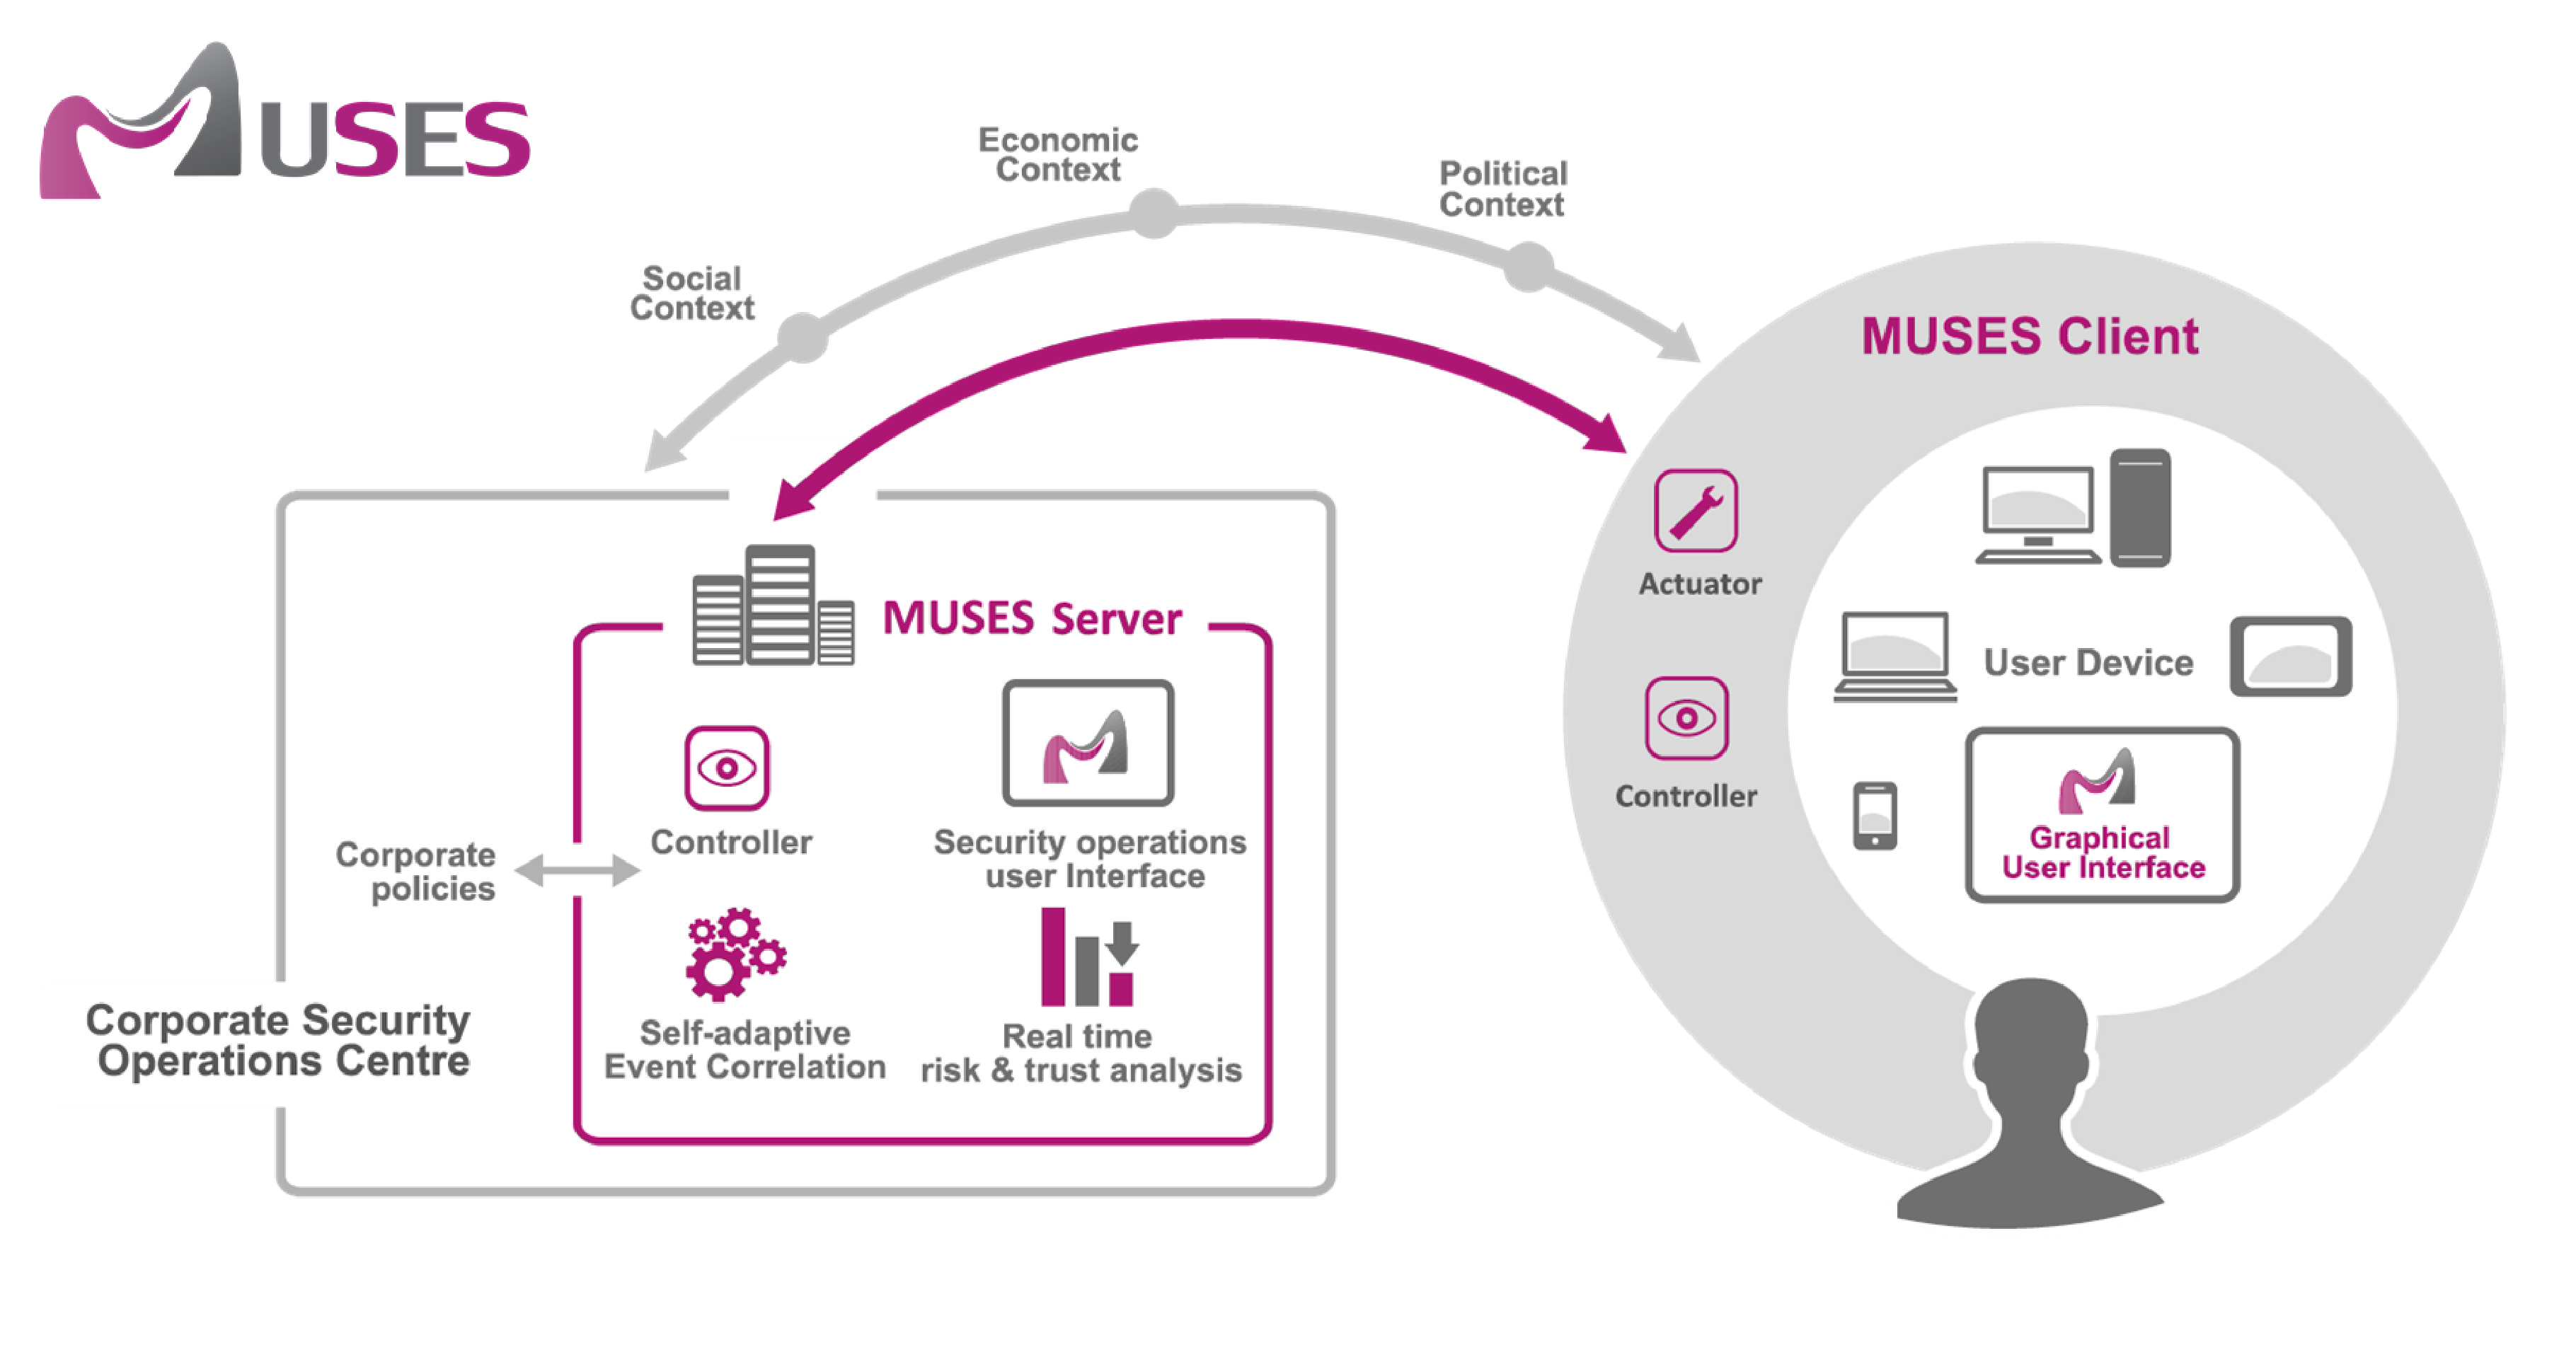
\includegraphics[scale=0.2]{img/system_overview.eps}
\caption{MUSES system overview. Conceptual model designed by S2 Grupo.  http://www.s2grupo.es/.\label{fig:system_overview}}
\end{figure}

As a summary, this application includes two modules: a \textit{controller} and an \textit{actuator}. The first one monitors the environment (context) and the users' behaviour, translating their actions in a sequence of events. These events, along with the patterns defining the user's conduct, are processed by the system in real-time by means of a Risk and Trust Analysis Engine (RT2AE) and an Event Correlation module. Then, a decision is taken in the corporate Security Operations Centre (SOC) side, considering the RT2AE output and the set of security rules adapted to that specific user and context. The corresponding feedback is communicated to the user through the \textit{actuator}, and then the user decides to comply or not with the policy. As was mentioned before, MUSES depends on the MUSES Aware applications to be able to really stop the application if the risk is dangerously high. In case that MUSES cannot kill the application process, and if the user decides to continue performing a risky action, the user trust value will decrease.

The designed MUSES architecture is shown in Figure \ref{fig:architecture}. It is a \textit{client/server} approach in which the \textit{client} application can be installed in every user's mobile or portable device, independently of the platform. On the one hand, MUSES client has been developed for Android, to be used in Android smartphones and tablets, as well as for Windows, so it can be used in Windows devices and laptops, and finally, iOS client will be also developed. On the other hand, MUSES server has been developed in Java, and works with an Apache Tomcat server. The \textit{server} side can be installed in the corporate server. Both sides are connected through a secure channel (using HTTPS) over the Internet. In that figure just the high-level components in each part are shown, along with the way the information flows in the system. %FERGU: esto no se si es de muses y posiblemente est� por terminar, pero quitad las comillas raras

\begin{figure}[ht]
%\begin{center}
\hspace{-0.7in}
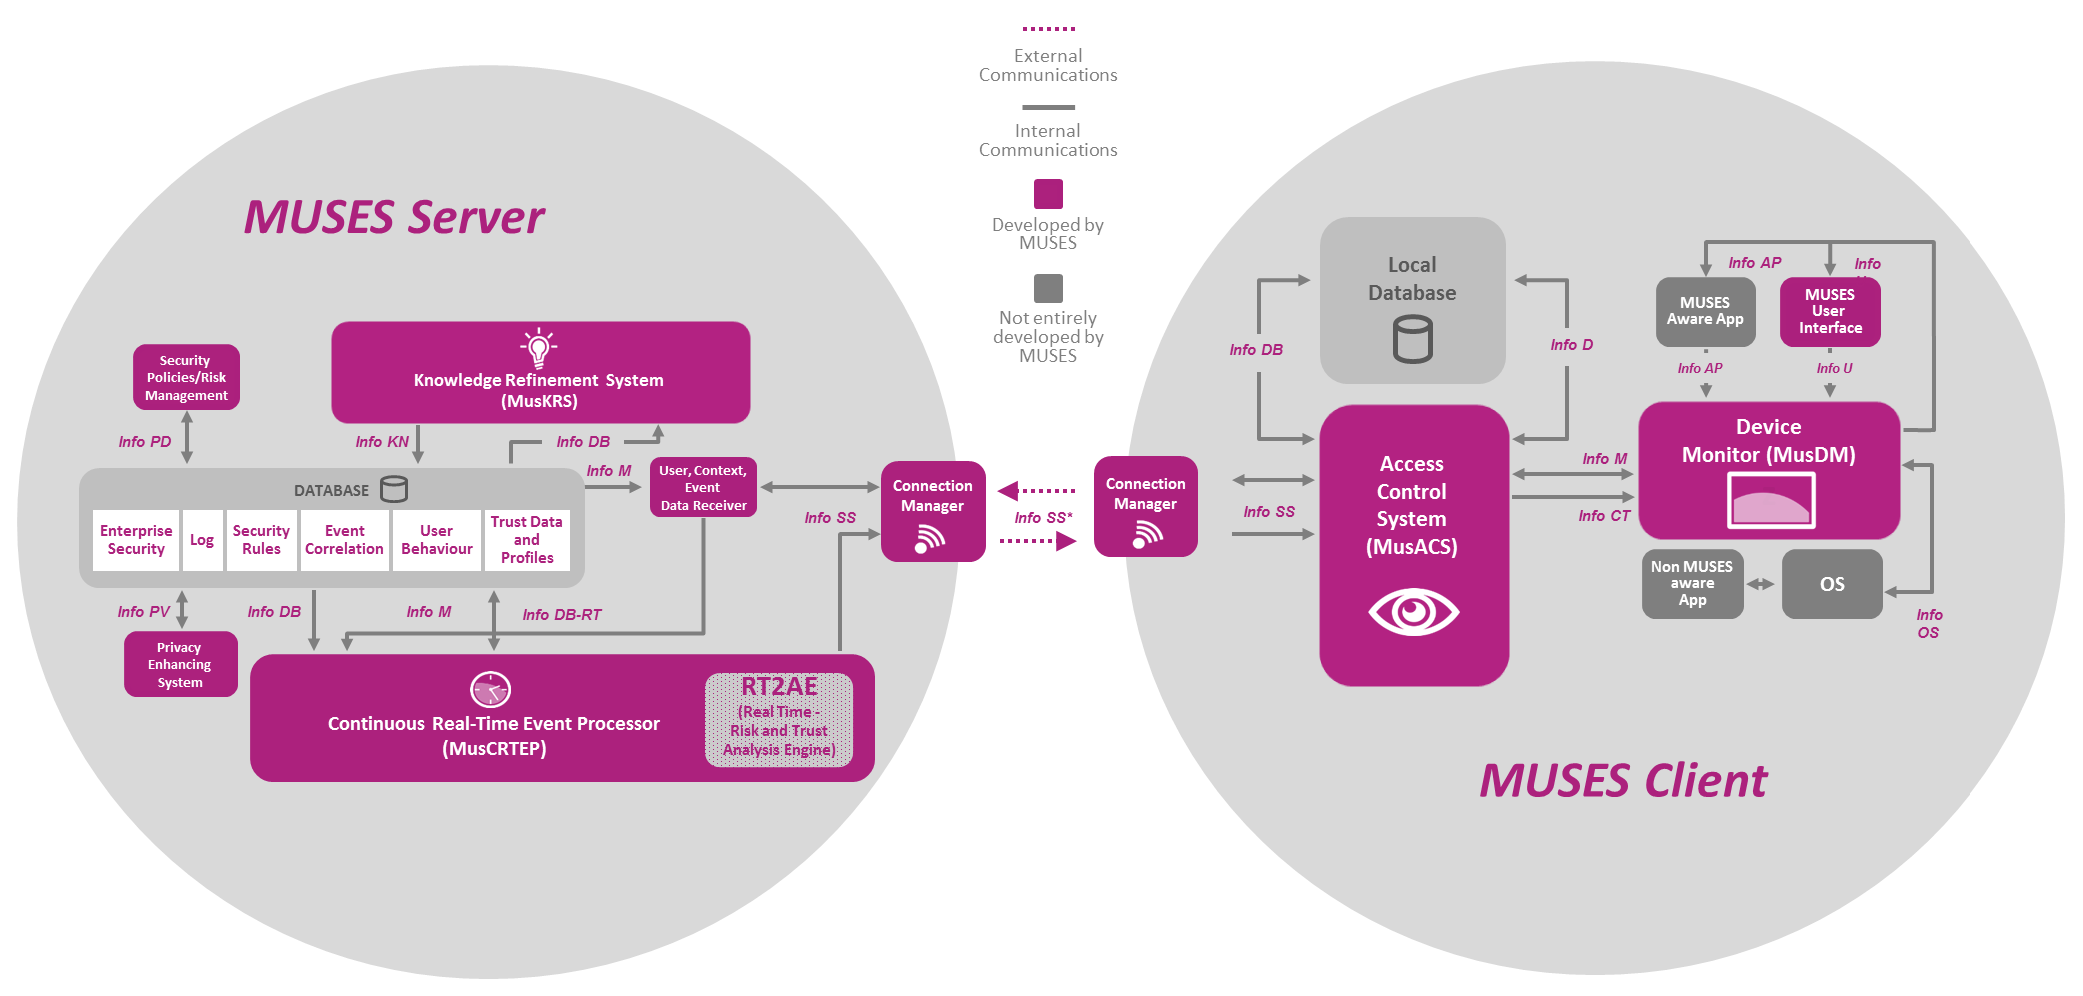
\includegraphics[scale=0.45]{img/architecture_modules.eps}
%\includegraphics[scale=0.45]{img/muses_architecture.eps}
\caption{Design of the MUSES architecture (art by S2 Grupo). \label{fig:architecture}}
%\end{center}
\end{figure}

The use of a server is mainly based on the need of a powerful machine, able to work with massive amounts of data (\textit{Big Data}) \cite{BigData_11}, since the algorithms to apply to them require high computational costs \cite{Shirkhorshidi14Review}.
Moreover, part of the high computational cost methods to apply needs to be derived to this high-performance server, as the mobile devices do not count with enough computational power. These methods include Data Mining \cite{DataMining_Lee01} and Machine Learning \cite{MachineLearning_Bishop06} techniques, which have been proved to be computationally expensive \cite{Cios07DataMining}. This server is also devoted to centralise the data gathering from all the devices in the company, composing a big database to which the commented techniques can be applied.

The system considers two working modes for every device: online and offline. In the \textit{online} mode the device can connect with the MUSES server, so that it can request the server to make a decision. On the other hand, in \textit{offline} mode the server cannot be reached by the device because there is not an available connection between them, so all the decisions are made locally.
This is done using an up-to-date copy on the Decision Table inside the Local database, which contains decisions for any type of detected event, along with the default actions to be performed if no rule is met. Anyway, in this mode, the gathered information by the sensors in the device is stored for later submission to the server side (when a connection is available), in order to be processed in the knowledge refinement process.
Moreover, when switching from offline to online mode, the device  receives an updated copy of the Decision Rules (the so-called Device Policies), as a kind of antivirus database, in order to work again perfectly in offline mode (if the connection is lost).

All flows of information in MUSES are encrypted with AES with 128-bit key in GCM mode \cite{viega2005use}, following the recommendations fo the Fact Sheet on Suite B Cryptography \cite{salter2012suite}. Also, the MUSES server authenticates to the MUSES client by means of a self-signed certificate. The authentication of the users is based on Spring Security, which is a Java/Java EE framework that provides authentication, authorization and other security features for enterprise applications. And finally, MUSES makes use of the fact that current operating systems for mobile devices provide encrypted data containers by default, like the feature used in Android Work. 

% ----------------------------------------------------------

\subsection{Client/Device architecture}
\label{subsec:client}

There are three main components in this side:
\begin{itemize}
 	 \item \textit{Local Database}: it is a local security-based storage, which includes the set of security rules to be applied locally (Device Policies), user authentication data, and a cache of gathered events and information. The latter is useful when the device is in offline mode, so these data are stored to be later submitted to the server side. 
%It contains the so-called \textit{Decision Table}, a set of rules in which the antecedents are high-level events, and the consequents are the corresponding decisions/actions, namely `allow', `deny' or `request' (the decision must be made in the server side).
 	 \item \textit{Device Monitor (MusDM)}: module which gathers the events and information produced by the user. It also acts following the decisions made by the system, in order to allow or deny the controlled application (or the user) for doing something. It is composed by a monitoring and an actuator submodules.
 	 \item \textit{Access Control System (MusACS)}: module in charge of making the decisions considering the gathered data. These decisions can be made locally (if possible), or can be requested to the server (if there is no rule which matches with the occurred events). 

%The subcomponents are the \textit{Decision Maker}, which performs the decision process; the \textit{User, Context, Event Handler}, which processes the events and information to be used for making the decision or stored for further submission (depending on the mode and on the gathered data); and the \textit{Security Policy Receiver} that updates the set of decisions (or Device Policies) in the Decision Table with those received from the server side, after an update or decision process.
\end{itemize}

As a clarification, there are several sensors implemented in the system. A \textit{sensor} is an application which monitorizes one type of interaction between the users and their devices. For instance MUSES includes a \textit{CONNECTIVITY SENSOR}, able to detect if the device has the WiFi or the Bluetooth enabled, if it is connected, if so, the BSSID of the network to which it is connected, the type of encryption, if the airplane mode is on, or the device's IP. 

There are also \textit{actuators} in the system, which are applications in charge of doing something on the monitorized user's actions, normally showing a message according to the decision made by the system, but which could sometimes act over some specific features of the device. For instance, in the previous example there is also a related actuator, which could restrict the connection to some networks, or activate the airplane mode, if required.

Some other examples of sensors are: DEVICE PROTECTION SENSOR (checks if the device is rooted, if it is protected by a password, or if there is an antivirus running), LOCATION SENSOR (detects if the device is within a secure zone), or a MAIL SENSOR (able to recognize the contents of an e-mail: from, to, cc, subject, attachment), among others.

The rest of the components shown in the figure are: the \textit{MUSES User Interface (UI)}, the application through which the user interacts with the system; and the \textit{Connection Manager} which controls the communications between client and server sides. 
In addition, there are two types of applications considered in this system: on the one hand the \textit{MUSES Aware App}, which is an application adapted to MUSES, so the system can directly interact with it (monitoring with the sensors and acting as a consequence of the decisions made by the system). This application must be implemented using the MUSES API (Application Program Interface)\footnote{The MUSES API is defined in the project, so for every application desired to be MUSES Aware, it should be implemented using this.}. 
Some of the commented sensors require the interaction with MUSES Aware Apps, in order to request for information. For instance, the MAIL SENSOR could not detect or recognize the contents of an e-mail unless the mail application provides them (so this must be MUSES Aware).

On the other hand the \textit{Non MUSES Aware App} is that which MUSES cannot directly interact with. Usually it can be accessed through the operating system (OS). So the type of information to gather from them and also the type of actions to do over them vary depending on the OS. In most of the cases MUSES could just detect/recognize very specific events, and also do very limited actions to prevent or block them (maybe showing a screen on the top until something is accomplished by the user). This is due to the usual denial or limitation of interactions with other applications that the OSs have. %FERGU: forbiddance parece que existe, pero el corrector me dice que no. Prohibition mejor?
% Yo dir�a que es forbidding...

% ----------------------------------------------------------

\subsection{Server architecture}

As in the client, there are three main components:
\begin{itemize}
	 \item \textit{System Database}: it stores all the information that the system can manage, including authentication data, enterprise security policies, assets' values, user-related information (trust, context), events data, and, of course, security rules to apply (with regard to the security policies).

	 \item \textit{Continuous Real-Time Event Processor (MusCRTEP)}: this component is the core of the MUSES system with respect to the decision making process. It includes an \textit{Event Processor}, the module in charge of performing the event correlation process \cite{deliverable21, deliverable52}. This is done by a so-called `Event correlation engine', which is in charge of taking the user action events that are sent from the device client, and analyse them to look for an existing security rule that could be applied to the situation. The engine discovers that by analysing the context events which are sent with the user action event, so that a complete model of the risks can be built. The output of this module is an `access request' which is sent to the \textit{RT2AE}. It considers the information included in the access request, as well as other information such as trust data and profiles, assets' values, user reputation, or opportunity, to perform a risk and trust analysis task \cite{RT2AE_SOTICS13}. Finally, the RT2AE extracts the set of potential rules to consider in the analysed situation, and these rules are therefore transformed into decisions (or Device Policies) and submitted to those devices to which they apply.

	 \item \textit{Knowledge Refinement System (MusKRS)}: this module is in charge of analysing the information stored in the system database by means of Data Mining techniques, identifying relevant data, such as important patterns, key features, or security incidents. These are later processed for tuning up the existing set of rules, or for inferring new ones. The KRS component, along with the CRTEP, are what represent the extension of the state of the art in security solutions for a BYOD environment. 

\end{itemize}

There are some other components, namely: the \textit{Security Policies/Risk Management} tool, that lets the company's CSO to define and manage Security Policies and Rules in a friendly way. It also lets the management of risk-related information, useful for the RT2AE process, such as the assets' values. The \textit{Privacy Enhancing System} which is a module aimed to fit with the legal compliance of the system regarding the user's data anonymisation and retaining of these data in the system. There are three important points with relation to this matter \cite{deliverable72}. First, the data that the user provides to the system (such as name, or email) is only used for authentication purposes, so they are checked when the user logs in the system, but they are not used for Data Mining tasks. Then, the location of the device is never sent and stored in the database, but instead, there are a number of defined `zones'. What is checked is that the user is inside one of those zones of interest. For instance, a company might want to know if the user is inside or outside a zone defined as `company premises'. And finally, the use in MUSES of what is called as `soft limit' and `hard limit' \cite{deliverable72}. These limits exist to ensure the users that their data will not be kept longer than necessary. The soft limit is defined by the components that use the data (Event Processor, RT2AE, and Knowledge Refinement System) for decision making or rule refinement, but do not need that data anymore. In addition, the hard limit is provided by the law, in case that the employee leaves the company, or if there is a national law specifying a maximum data retention period.

Then, the \textit{User, Context, Event Data Receiver} is devoted to receive data from the device side (events, or user-related data, among others) and to distribute them among the components (storing in the database, and requesting the Event Processor to start the correlation task). Finally, there is another \textit{Connection Manager} which controls the communication with the device side. %FERGU: no usar etc en art�culos, mejor poner: (events, user-related LOQUESEA, among others)
% Cambiado


% ----------------------------------------------------------

\subsection{Self-Adaptation in MUSES: The Knowledge Refinement System}

As previously stated, one of the main features of this system is the self-adaptation (to the user and context), of the set of Corporate Security Rules (specification of the ISPs), that it is be able to perform. 
To this end, the \textit{MusKRS} module is run asynchronously in the server (once a day or every X hours) and it is in charge of analysing all the gathered information (events, context, user-related data), and adapting/refining the security rules. The refinement (improvement)  has as aim to better deal with these events, optimizing the current set of rules (removing redundant or non-useful rules, for instance), and even trying to predict future threats due to the user's behaviour.

This procedure is be composed by two main steps: first, a Data Mining (DM) \cite{DataMining_Lee01} + Machine Learning (ML) \cite{MachineLearning_Bishop06} process is performed (in the \textit{Data Miner} sub-component);  second, a refinement and inference process  is done (in the \textit{Knowledge Compiler} sub-component), considering the data `extracted' in the first step, by means of Computational Intelligence (CI) techniques.
It should be noticed that part of the refinement (or adaptation) of the security rules is made using simpler methods, such as generalisation or specialisation of rules, for instance. Then, other parts of the process can be conducted using CI.

Another important fact is that MUSES  counts with a human controller, normally the Chief Security Officer (CSO) of the company, who  supervises the system activity by means of logs or feedback messages. Thus, adapted and inferred security rules are not, in principle, directly added to the current set of rules. Instead, they  are proposed as draft rules to this controller, in order that he/she can accept them if they are interesting and correct. The system  is able to `learn' from this decisions, so after a so-called training or `warm up' period, the rules can be directly accepted (included in the set) or rejected autonomously by the MusKRS.

The following sections describe these processes: first focusing on DM techniques to be used both automatically by the MusKRS, and as a kind of decision-aid/monitoring tool for the CSO; second, the CI techniques are explained, mainly focusing in Evolutionary Computation (EC) \cite{EAs_Back96} approaches, since these methods perform very well, and have been widely used in security-based environments for solving security issues, such as the intrusion detection \cite{GA_intrusion-majeed}, the design and evaluation of security protocols \cite{GP_intrusion-lu,GA_networksecurity-zarza}, or the optimisation of different aspects related with security: IT security costs \cite{EAs_securitycosts-kirta}, and cryptographic protocols \cite{GA_cryptographicprotocols-zarza2}, among others.

% ------------------------------------------------------------------
%
\subsubsection{Data Mining + Machine Learning}
\label{subsubsec:dm_ml}

This task is performed by the \textit{Data Miner} module. It  takes the `raw' data from the database and  process the information, in order to yield a set of relevant data for the Knowledge Compiler module or for the human controller. In the first case, this sub-component  takes them as a reference in order to refine or adapt the current set of security rules (for instance, to deal with anomalous situations).

The process is be mainly non-supervised. Moreover, eventually, the datasets can be huge (depending on the company's data flows), so Big Data processing methods \cite{BigData_11} can be applied.

The DM/ML techniques process the so-called patterns, which in this context correspond to events (and their related information) produced by the users' interactions with the system. As stated, these events  are captured from the sensors in the users' devices and transmitted to the server to be processed and stored in the system database. The methods to be applied are:

\begin{itemize}

\item \textit{Pattern Mining} \cite{PatternMining_Han07}: 
This process  tries to identify frequent or, on the contrary, anomalous patterns, in order to process them lately. The idea is that non-frequent patterns are potentially suspicious, and thus, could be of interest to be checked by the CSO or to serve as a reference for the rule-refinement process.

\item \textit{Classification} \cite{classification_67}: 
This technique tries to train a model (classifier) able to associate every pattern in the dataset to a class, so that the model could be used for assigning a class for further incoming patterns with an unknown category.
For instance, it could look for events (patterns) that had been previously  marked as `allowed' or `denied' (according to the ISPs). When a new event arises, if it has not an assigned decision, the classifier should provide one based on the similarity with previous (and already labelled) patterns.

\item \textit{Clustering} \cite{Clustering_Jain99}: 
The aim of this method is grouping the patterns considering some similarity criteria, in order to manage them as a set. This could be used for providing data visualisation mechanisms, in order to make it easier to interpret the data interaction and the distribution in clusters with respect to the different properties/features of the patterns.

\item \textit{Feature Selection} \cite{FeatureSelection_Guyon03}: 
It consists on extract the most important features/variables from the data. This could be useful if we want to discard non-key features, which could be interesting in order to reduce the database weight, for improving the performance of other techniques (such as classification or clustering), and even to improve the performance of the whole system, since less information would be gathered and transmitted.

\item \textit{Data Analysis}: 
This  provides the CSO with mechanisms to visualise interesting facts about the data, such as more frequent events, dangerous or suspicious users (according to their behaviour), more triggered rules, etc.

\end{itemize}

%\pagebreak

% ------------------------------------------------------------------
%
\subsubsection{Computational Intelligence: Evolutionary Computation Methods}
\label{subsec:ci}


MUSES  uses different EC approaches, initially, two in the DM/ML part of the process, and three in the rule-refinement/adaptation phase. They are based on Genetic Programming (GP) \cite{GP_Koza92}, and Genetic Algorithms (GAs) \cite{GAs_Goldberg89}.

The first evolutionary-based approach is a \textit{GP-based classification} method. This is useful for two main reasons: first, in order to deal with the data class imbalance \cite{imbalance_techniques_02}, very common in classification problems in real systems (with real data); and second, to better manage categorical (non-numeric) data, since most of the features/variables and information gathered from the events take these kind of values.

Thus, this approach is be able to manage unbalanced datasets considering a fitness function in which a cost can be associated with the classifier accuracy at every epoch, having a penalty cost when the classifier makes a false negative (an element from the minority class which is classified as belonging to the majority class) \cite{cost_adjustment_07}.
Regarding the type of data, since GP algorithms can manage rule- or tree-based models, it  works perfectly with any categorical variable, yielding a good classifier as it has been made in other works (such as the aforementioned \cite{cost_adjustment_07}).

The second approach is a Feature Selection process, conducted using a GA as a meta-algorithm to test all the possible combinations of pattern features/variables in the classification. Thus, the algorithm can optimize the group of features to be considered in the classification task, improving both the computational time of this task and also the obtained accuracy of the method.

The second set of EC techniques is, as stated, part of the rule-refinement (or adaptation) process, to be performed by the \textit{Knowledge Compiler} module. These methods can be used for inference and optimisation, and consider this data as a part of the process:

\begin{itemize}

\item The information extracted from the Data Miner sub-component, mainly concerning the anomalous, unclassified or misclassified patterns. These are those patterns which did not match with any of the existing classes (they are quite different from the patterns belonging to those classes), so they cannot be included in any of the classes and thus they should be taken into account for a potential inference or update in the set of security rules, in order to `cover' them.

\item User-related information corresponding to those anomalous or unlabelled patterns (events). Thus, the user's ID, location and role, for instance, can be considered in order to select the applicable set of rules for that conditions.

\item Context information for the same patterns, in order to also restrict the applicable set of rules considering this information. 

\end{itemize}

Other useful information to consider in the refinement/ adaptation process are:

\begin{itemize}

\item Risk information extracted from the user profile (user trust value), e.g. ``Did the user received a lot of `denies'/`allows' before?'', i.e. ``Is the user trustworthy?''. In case the user is not, more restrictive rules can be created, otherwise the corresponding rules could be `relaxed' for that user.

\item The information stored in logs along the system, which can, for instance, tell about how the user responds to system messages (either an action or if the user gives feedback). This could result in the inference of new rules or in adaptation, in order to deal with, for instance, users that repeatedly ignore warning messages.
Moreover, important log information regarding the parameters used or the decisions made in the different modules can be used for further tests of new inferred rules, as it is explained below.

\end{itemize}

This being said, and because the refinement of rules is considered of the same importance as inferring new ones, the approaches that have been implemented are:

\begin{itemize}

\item \textit{GP rule inference} method, which generates/creates new rules in order to `cover' those situations non contemplated in the current set of rules. Thus, for instance, a new rule could be created in order to deal with the patterns to which the classifier could not assign a class.
The generation can be done considering the so-called \textit{dictionary}, i.e. a set of terms corresponding to all the possible inputs and actions in the system, which are antecedents (conditions) and consequents in the security rules to be inferred.
The evaluation of these rules can be done considering the stored log information concerning the parameters along with the actions/decisions made in every component in the system. Thus, it is possible to `simulate' the whole  system behaviour when the new rule is included and get a value of its performance.

\item \textit{GP rule refinement} approach, which optimises the current set of rules, adjusting the values in the conditions (antecedents), for instance. Thus, some superfluous parts of the rules and even complete rules could be removed or improved, obtaining for instance specialisations or generalisations of existing rules which could mean a better performance.
The evaluation (of the whole set of security rules) is done considering the number of unlabelled patterns that are `covered' after the adjustments.

\item \textit{GA optimisation} algorithm for setting up and adapting the assets' values. These are numerical representations of the importance of the corporate assets, and are considered in the Real-Time Risk and Trust Analysis process, in order to assign a risk value to every potential decision that can be made by the system.
If it is possible to evaluate the partial solutions proposed by the GA, this approach could be very useful for the CSO (who is in charge of assigning and adjusting these values over time).
The adaptation or adjustment concerns the change in value that an asset could have due to a loss of importance, once an event has passed (a project presentation, for instance).

\end{itemize}


%----------------------------------------------------------------------------
%%%%%%%%%%%%%%%%%%%%%%%%%%%%%%%   COMPARISON  %%%%%%%%%%%%%%%%%%%%%%%%%%%%%%%
%----------------------------------------------------------------------------

\section{MUSES Advantages over Other Solutions. Beyond the State of the Art}
\label{sec:comparison}


MUSES is mainly a free, open-source, platform independent solution, and that makes it a very good option in a first comparison against most of the proprietary, close and system-specific tools presented in Section \ref{sec:toolsreview} (all but WSO2). In addition, most of the existing tools take into account only smartphones and tablets, but MUSES also  covers laptops and company PCs too, thus, it is not only for BYOD. Moreover, the companies which might want to work with one of the reviewed systems need a specific operating system in the server (such as Windows Server, for instance), being even more restrictive in some cases. This is specially remarkable in the case of the Blackphone, forcing the companies and the employees to purchase a specific device. MUSES is a good solution towards these cases, since it is a multiplatform system in both the client and the server. 

Another comparison would be that the existing products are mostly policy-based, while MUSES makes its decisions not only considering policies, but also based on the terminals/users context (connection properties, or trust value of the device, for instance), to really understand the real risk that comes with a specific action.

Also related to this issue, a very big plus of the MUSES system (not present in the other solutions) is its self-adaptivity power. Thus, MUSES is able to adapt to changes, either regarding corporate security policies, newly discovered vulnerabilities or threats, different environments of use, or user profiles. 

Moreover, another clear advantage over the rest is that MUSES can work in both online and offline modes, depending on the client being able to connect with the server or not, which favours a real-time decision making process.

These are not only advantages of MUSES over the existing products, but also a progress beyond the state of the art in some fields like risk and trust analysis, event correlation, and human-computer interaction (HCI).

First, as mentioned previously, it  implements a self-adaptive event correlation, including a novel hybrid technique of rule refinement and rule adjustment extracting relevant information from processing huge amounts of data. Then, the project defines a new approach to risk management taking into account threats (with their costs) as well as the innovative concept of opportunity, i.e. the following beneficial outcome from a situation on which, for instance, a user is able to work while waiting at the airport if the risk is low enough. 

About HCI and usability of mobile devices, this sets up a significant advance in the state of the art because of the novelty of the BYOD philosophy, and trying to look for individual differences among the users in susceptibility to persuasive strategies for secure behaviour. Regarding device monitoring, MUSES  also take into account the so-called context observation, by which private or professional scenarios can be detected, or predicted, based on advanced machine learning techniques. Finally, the project is concerned about legal compliance in regards of Information Security Policies, so that it  contributes to the proposal for the EU Data Protection: legal binding force and legal certainty of company policies, and end-user responsibility.

With regard to the scientific contribution of the system, one of the main differences with respect to previous works is the consideration of security threats `brought' by the user's behaviour inside the system, i.e. through interaction/events, rather than more general and external threats. Moreover, the techniques to be used in MUSES  works with real data (in a real system), as a difference to several research works (they consider simulated or artificial data).

Data Mining techniques have been used by the authors in some works, but usually aiming for a specific general objective, for instance the detection of threats (botnet) \cite{botnet_detection_clustering_09}, or the recognition of anomalies \cite{feature_selection_anomalies_08}, but they are not linked with a following process to improve the system (the refinement phase in MUSES).

There are some proposals in which security policies are inferred or refined \cite{inferring_policies_socialnetworks_09,policy_generation_clustering_10}, but they do not affect the ISPs as in MUSES, and they are not based on the user's behaviour in order to do this.

Genetic Programming has been previously used by several authors \cite{rule_generation_gp_09,sec_policy_evolution_gp_08}, even for creating new policies or rules in a security-aimed sense, but they do not affect the ISPs and moreover, our proposed evaluation functions (completely integrated in the system) for the refinement and inference approaches are novel.

With respect to Genetic Algorithms, they have been extensively used in this scope in the literature, mainly for the detection of anomalies and intrusions rather than for optimisation, as in our case. However, there are some examples that could be used as model for our approach, such as \cite{EAs_securitycosts-kirta,risk_reduction_ga_12}.

	
%*** Features:
%Concept of framework-enabled app (Citrix' Worx-enabled apps == MUSES-aware app)
%
%*** Azzurri includes several of the MUSES features


%\begin{table}
%{\tiny
%\begin{tabular}{cllllll}
%\hline
%\multicolumn{1}{|c|}{\textbf{Feature}} & 
%\multicolumn{1}{c|}{\textbf{Muses}} & \multicolumn{1}{c|}{\textbf{\begin{tabular}[c]{@{}c@{}}IBM\\ Mobile\\ Security\end{tabular}}} & \multicolumn{1}{c|}{\textbf{\begin{tabular}[c]{@{}c@{}}Sophos\\ Mobile\\ Control\end{tabular}}} & \multicolumn{1}{c|}{\textbf{\begin{tabular}[c]{@{}c@{}}Samsung Knox\\ and\\ Blackberry Balance\end{tabular}}} & 
%\multicolumn{1}{c|}{\textbf{Blackphone}} & \multicolumn{1}{c|}{\textbf{\begin{tabular}[|c]{@{}c@{}}Android\\ for\\ Work\end{tabular}}}\\
%\hline
%License                                                           & Open Source                         & Proprietary                                                                                    & Proprietary                                                                                      & Proprietary                                                                                                    & Proprietary                                                           & Proprietary\\
%\begin{tabular}[|c]{@{}c@{}}Devices\\ \&\\ Platforms\end{tabular} &                                     &                                                                                               & \begin{tabular}[|c]{@{}l@{}}IOS, Android\\ and Windows Phone 8\end{tabular}                      & \begin{tabular}[|c]{@{}l@{}}Android Samsung devices\\ and IOS\end{tabular}                                     & Own device                                                           & \begin{tabular}[|c]{@{}l@{}}Android and\\ Devices with \\ Chrome Browser\end{tabular}\\
%Price                                                             & Free*                               &                                                                                               & By request                                                                                      & 12\$ per year/device                                                                                          & \begin{tabular}[|c]{@{}l@{}}120\$ per \\ year **\end{tabular}         & \begin{tabular}[|c]{@{}l@{}}\$50 per user per month\\ \$12 per user per month\\ with unlimited storage\end{tabular} \\
%Strengths                                                         &                                     &                                                                                               & \begin{tabular}[|c]{@{}l@{}}Can manage countless\\ devices with one solution\end{tabular}        &                                                                                                               &                                                                      & \begin{tabular}[|c]{@{}l@{}}Cloud based\\ Integrated in Google for Work\end{tabular}                              \\
%Handicap                                                          &                                     &                                                                                               &                                                                                                 &                                                                                                               & \begin{tabular}[|c]{@{}l@{}}Only to their\\ own devices.\end{tabular} &                                                                                                                  \\
%\hline
%\multicolumn{7}{l}{\begin{tabular}[c]{@{}l@{}}\textit{* Requires own hardware}\\ \\ \textit{** By purchasing the terminal tree one-year subscriptions are archived}\end{tabular}}                                                                                                                                                                                                                                                                                                                                                                                                                                                  
%\end{tabular}
%}
%\end{table}


%----------------------------------------------------------------------------
%%%%%%%%%%%%%%%%%%%%%%%%%%%%%%%   CONCLUSIONS  %%%%%%%%%%%%%%%%%%%%%%%%%%%%%%%
%----------------------------------------------------------------------------

\section{Conclusions}
\label{sec:conclusions}

This work introduces a self-adaptive user-centric end-to-end system, named MUSES. The first prototype of this system has been recently released, and it has been already tested in an actual company, with excellent results and very positive feedback. The architecture and main features of the system are described, paying special attention to the application of Soft Computing methods in tasks of data analysis, machine learning, and also in the use of evolutionary algorithms to improve the existing set of corporate security rules which leads the system. %Antares - Yo podr�an en lugar de ``next year'' el a�o, porque el art�culo puede ser le�do en cualquier momento y es mejor emplear referencias absolutas, �no creeis? FERGU: fuera

MUSES has been compared with other existing solutions/tools with a similar aim: to ensure the protection and privacy of sensitive information in the enterprise when it is accessed by the employees using their own devices (BYOD philosophy).
The main advantages of MUSES with respect to the other solutions have been discussed, also remarking its advances beyond the state of the art that define these tools.

In addition, a scientific comparison between the techniques used in the presented system and those in the literature, in the same scope, has been done. It has been discussed that MUSES has the advantage of being multiplatform, while most of the reviewed tools are not. In addition, MUSES is able to adapt and evolve the security policies that a company has built, and not only apply them, as the other tools do. Also, it is remarkable that this MUSES tool is not a solution offered by a company, but the result of the aim of going beyond the state of the art in different fields of research.
	
However, there is room for considering some of the existing researches that could be added as future features for MUSES, such as the analysis of users via social networks \cite{inferring_policies_socialnetworks_09,user_classification_ml_13}, the optimisation of security protocols \cite{GA_networksecurity-zarza}, the implementation of intrusion detection mechanisms \cite{GA_intrusion-majeed}, or the application of novel privacy-related techniques \cite{AAI_book_2009}, which is another feature also considered in MUSES. The second prototype of the system will be also released, as well as the conclusions extracted after the analysis of data from the test of the first prototype.


%%%%%%%%%%%%%%%%%%%%%%%%%%%%%  ACKNOWLEDGEMENTS %%%%%%%%%%%%%%%%%%%%%%%%%%%%%%%%

\section{Acknowledgements}
This paper has been funded in part by European project MUSES
(FP7-318508), along with Spanish National projects
TIN2011-28627-C04-02
(ANYSELF) and TIN2014-56494-C4-3-P (EphemeCH), and GENIL PYR-2014-17,
awarded by the CEI-BioTIC UGR.  

\bibliographystyle{elsarticle-num}
\bibliography{review_muses,geneura-latin1}

\end{document}
%%% Local Variables:
%%% ispell-local-dictionary: "english"
%%% hunspell-local-dictionary: "english"
%%% End:
